\documentclass[output=paper
,modfonts
,nonflat]{langsci/langscibook} 


\title{Distributed agreement in participial sandwiched configurations} 
\author{Franc Lanko Marušič\affiliation{University of Nova Gorica}\lastand Andrew Nevins\affiliation{University College London}}
% \chapterDOI{} %will be filled in at production
% \epigram{}

\abstract{In recent years, several proposals have appeared that try to model the patterns of agreement with coordinate noun phrases found in South Slavic Languages. We investigate agreement in so-called `sandwiched' configurations, whereby a coordinated noun phrase sits between two agreeing participles. In such cases, the two participles do not necessarily agree with each other, given a scenario in which the first and the second conjunct have different phi-features. This means the two participles choose their target of agreement independently. We argue the results of our experimental study favor an approach to agreement that places it partially in PF.}

\begin{document}
\maketitle
\section{Introduction} 

South Slavic languages allow three possibilities for agreement with coordinate noun phrases: highest conjunct agreement (HCA), closest conjunct agreement (CCA), or default agreement (masculine), as shown in (\ref{initial})--(\ref{initial2}) for Slovenian (where not explicitly noted, all examples are from Slovenian).

\begin{exe}
\ex \label{initial}
\gll Krave in teleta so odšla / odšle / odšli na pašo.\\
cow.\textsc{f.pl} and calf.\textsc{n.pl} \textsc{aux.pl} went.\textsc{n.pl} / went.\textsc{f.pl} / went.\textsc{m.pl} on graze\\
\glt `Calves and cows went grazing.'
\ex \label{initial2}
\gll Teleta in krave so odšla / odšle / odšli na pašo.\\
calf.\textsc{n.pl} and cow.\textsc{f.pl} \textsc{aux.pl} went.\textsc{n.pl} / went.\textsc{f.pl} / went.\textsc{m.pl} on graze\\
\glt `Calves and cows went grazing.'
\end{exe}
Following our previous work on closest-conjunct agreement in South Slavic \citep{marusicnevinssaksida:07,marusicnevinsbadecker:15,willergold:16}, in the present paper we investigate so-called `sandwiched' configurations, whereby a coordinated noun phrase sits between two agreeing participles, as in (\ref{sand}).\footnote{\citet{bhattwalkow:13} provide a similar case of agreement in sandwiched configurations in Hindi/Urdu, for which they claim disagreeing choice of goals is not possible. We have found some variability in informal consultations with native speakers, and contend that the possibility of finding a parallel with Double CCA in Slovenian within Hindi/Urdu awaits further study.} In this example, each participle exhibits Closest Conjunct Agreement (CCA) in gender with the conjunct linearly closest to it:

\ea \label{sand}
\gll Včeraj      so    bile       [ krave    in    teleta ]    prodana.\\
yesterday \textsc{aux.pl} been.\textsc{f.pl} {} cow.\textsc{f.pl} and calf.\textsc{n.pl} {}   sold.\textsc{n.pl} \\
\glt `Yesterday cows and calves were sold.' \citep{marusicnevinsbadecker:15}
\z
The relevant structures are those with either [feminine + neuter] or [neuter + feminine] coordinations, as this is a three-gender language, where masculine agreement plays the role of default gender in the plural \citep{marusicnevinsbadecker:15,willergold:16}. Default agreement is thus clearly diagnosed (i.e. masculine agreement with conjoined feminine and neuter nouns) in agreement configurations such as (\ref{sand}). In acceptability judgement studies carried out with native speakers of Slovenian, we found that Double CCA (i.e. each participle agreeing with the conjunct linearly closest to it) were most highly rated, followed by Double HCA (each participle agreeing with the first conjunct in the coordinate NP), as in (\ref{doublehca}):

\ea \label{doublehca}
\gll Včeraj so bile  [ krave in teleta ] prodane.\\
yesterday \textsc{aux.pl} been.\textsc{f.pl} {} cow.\textsc{f.pl} and calf.\textsc{n.pl} {} sold.\textsc{f.pl} \\
\glt `Yesterday cows and calves were sold.' 
\z
Still acceptable, though less so, was HCA on the first participle, and default agreement on the second participle, as in (\ref{highestdef}):

\ea \label{highestdef}
\gll Včeraj      so    bile       [ krave    in    teleta ]    prodani.\\
yesterday \textsc{aux.pl} been.\textsc{f.pl} {} cow.\textsc{f.pl} and calf.\textsc{n.pl} {}   sold.\textsc{m.pl} \\
\glt `Yesterday cows and calves were sold.' 
\z
However, structures that exhibited default agreement or furthest-conjunct agreement by the highest participle were rated as unacceptable:

\begin{exe} 
\ex
\begin{xlist}
\ex \gll *Včeraj      so    bili       [ krave    in    teleta ]    prodana.\\
yesterday \textsc{aux.pl} been.\textsc{m.pl} {} cow.\textsc{f.pl} and calf.\textsc{n.pl} {}   sold.\textsc{n.pl} \\
\glt `Yesterday cows and calves were sold.' 
\ex \gll *Včeraj      so    bili       [ krave    in    teleta ]    prodani.\\
yesterday \textsc{aux.pl} been.\textsc{m.pl} {} cow.\textsc{f.pl} and calf.\textsc{n.pl} {}   sold.\textsc{m.pl} \\
\glt `Yesterday cows and calves were sold.' 
\ex \gll *Včeraj      so    bila       [ krave    in    teleta ]    prodana.\\
yesterday \textsc{aux.pl} been.\textsc{n.pl} {} cow.\textsc{f.pl} and calf.\textsc{n.pl} {}   sold.\textsc{n.pl} \\
\glt `Yesterday cows and calves were sold.' 
\end{xlist}
\end{exe}
These results have clear theoretical consequences for arbitrating between extant theories of South Slavic conjunct agreement, as they show that linear order must be present in order to accomodate cases of Double CCA. \cite{marusicnevinsbadecker:15} and \cite{willergold:16} present a distributed theory of conjunct agreement, whereby each agreement target (Probe) identifies its domain of agreement controllers (the Goa) within syntax, but carries out the actual copying of features from Goal to Probe at PF, at which point linearity is present. This approach therefore follows the two-step Agree operation outlined in  \citet{arregi-nevins:12}, see also Chapter 1: Sec 2.3 and \citetv[Section 4]{chapters/05-kalin.tex} for discussion of the timing of Agree across components: with Agree-Link in the syntax, and Agree-Copy in PF. Agree-Link establishes a relation between a participle and a Goal (i.e. the subject \&P), whereas Agree-Copy actually enacts the work of copying the features from Goal to Probe. Crucially, operations such as Linearization of the syntactic structure (at which point linear order becomes available) may be interleaved between these two. When Linearization feeds Agree-Copy, CCA results. 

If Agree-Copy takes place before linearization, all copying must respect HCA, as by hypothesis, only hierarchical structure is present. On the other hand, if Agree-Copy takes place after linearization, all copying is done with the closest conjunct to each participle. Default agreement -- i.e. agreement with the head of \&P itself --  when it takes place, is a restricted option, one possible only when the \&P c-commands the participle (\citealt{willergold:16}, following \citealt{smith:17a}) and hence unavailable postverbally.

For sandwiched configurations, assuming that each participle establishes Agree-Link with the conjoined subject noun phrase, if Agree-Copy takes place after linearization, then each participle will copy the values for agreement from the linearly closest conjunct within the \&P to it. Whether Agree-Link itself is upward or downward for the subject noun phrase and each of the two participles is not directly relevant for Double CCA, as all that matters is the relative linear position of each conjunct with respect to each participle once Agree-Copy applies. Agree-Link is always established with \&P alone, and once Agree-Copy fails to find lexically-supplied gender features at the \&P level (when default values are not chosen), Agree-Copy must take a value from one of the conjuncts inside the \&P -- either highest or closest, depending on the timing with respect to Linearization.

Other models of conjunct agreement do not fare so well with respect to the sandwiched configurations. In particular, \citet{puskarmurphy:17} have a theory of conjunct agreement in which all agreement is computed internally to the \&P that heads the coordinated noun phrase. As such, there is no direct way for two agreement targets to choose different parts of the \&P. 
%new sentence
\citet{puskarmurphy:17} derive Double CCA pattern by invoking feature deactivation, proposing (in Section 5.1) that following agreement with the lower participle the features of the second conjunct, which were present at the \&P layer, can be deactivated and are thus invisible for agreement with the higher participle. As a result, the higher participle must take the values from the first conjunct, as this is the hierarchically closest conjunct. This derives Double CCA, but the same mechanism of deactivation would seem to pose problems for deriving Double HCA. For \citet{boskovic:09}, preverbal HCA is predicted not to exist in the first place, hence Double HCA as in (\ref{doublehca}) is impossible to derive. Equally impossible is the Double CCA pattern: for \cite{boskovic:09}, CCA is made possible by the deletion of the gender features on the first conjunct, but if the first conjunct has no gender features it cannot then agree with the higher participle.

The issue largely has to do with the problems that sandwiched configurations raise for syntax-internal timing. Appealing to feature deactivation in order to account for different patterning of the two participles (\&P’s features deactivated by Part$_2$, and hence Part$_1$ syntactically probes within the higher conjunct) is difficult to assess. They depend on the position of the \&P at the moment of probing (are both probes initially higher? Does Part$_2$ probe and trigger movement, and Part$_1$ only probes?). On the other hand, placing Agree-Copy in PF makes the surface order in sandwiched configurations all that matters for determining Double CCA/HCA. Agreement on the 1st participle mirrors the options available with postverbal subjects, while agreement on the 2nd participle mirrors the options available with preverbal subjects. The two agreement processes are carried out independently by each probe in PF.

\section{Sandwiched coordinated subjects}\label{sec:sandwconf}

We use the term `sandwiched configuration' for all cases of multiple agreement probes on opposite sides of the coordination phrase. One such case is presented above, repeated here as (\ref{sand2}), where two participles are placed on the opposite sides of the coordinated subject, in this case an \textit{l}-participle and an \textit{n}-participle\footnote{So-called \textit{l}-participles are verbal participles that are used in compound tenses and conditionals in both Slovenian and Bosnian/Croatian/Serbian (as well as in other Slavic languages). They are sometimes called active participles or simply past participles. Typically they are considered to be part of the verbal paradigm (\citealt{browne:93}, \citealt{priestly:93}). The \textit{n}-participles, on the other hand, also know as passive participles, are found in adjectival passives and are homophonous with adjectival forms (ibid.).} of an adjectival passive. In Bosnian/Croatian/Serbian, the equivalent of such cases are generally reserved for pluperfect constructions, as noted by Nadira Aljović (pers. comm).

\ea \label{sand2}
\gll Včeraj      so    bile       [ krave    in    teleta ]    prodana.\\
yesterday \textsc{aux.pl} been.\textsc{f.pl} {} cow.\textsc{f.pl} and calf.\textsc{n.pl} {}   sold.\textsc{n.pl} \\
\glt `Yesterday cows and goats were sold.'
\z
In principle, a sandwiched configuration is also a situation where the main auxiliary itself is located on the other side of the subject from the participle, but as the auxiliary in South Slavic languages does not agree in gender and the participles do not agree in person, the two elements seem to act as different kinds of probes: the auxiliary probes for number and person features, while the \textit{l}-participle probes for number and gender features. We do not discuss such cases  further here, and wish to reserve this term for instances where the two agreeing elements share every dimension of their agreement. In the present paper, in fact, we assume that auxiliary agreement is independent from participle agreement, precisely because the two have different specifications for which features they agree with (see \citealt{dalessandro:07}, \citealt{lopez:07}, \citealt{puskar:17}, among others, for discussion).

Another instance of a sandwiched configuration is presented in (\ref{whichtowns}), where a determiner showing gender and number agreement within the coordinated subject scopes over both nouns but precedes the first noun. At the same time, the participle sits on the other end of the conjunction. A fuller discussion of such examples can be found in \cite{begovicaljovic:15} and \cite{aljovicbegovic:16}. 

\ea \label{whichtowns}
\gll [ Katera [ mesta in vasi ]] so tekmovale?  \\
{} which.\textsc{n.pl} {} town.\textsc{n.pl} and village.\textsc{f.pl} {} \textsc{aux.pl} competed.\textsc{f.pl}\\
\glt `Which towns and settlements competed?'
\z
Similar to this partially-DP-internal case of sandwiched configurations is an instance of an adjective inside the subject, again preceding the first noun and showing gender and number agreement. Given the nature of the adjective in (\ref{togetherlying}), it can only structurally modify the two nouns in conjunction. The adjective is not simply  structurally part of the first noun phrase of the coordinated subject, but instead is a modifier of the entire coordination. When the participle follows such a subject, this yields another instance of a sandwiched configuration \citep{marusicetalnels:15}; see \citetv{chapters/03-carstens} for a discussion of shared mechanisms between NP-internal concord and Agree by verbal elements.

\ea \label{togetherlying}
\gll [ Skupaj  ležeča   [ vabila         in    reklame ]] so      pristale     v  smeteh. \\
{} together lying.\textsc{n.pl} {} invites.\textsc{n.pl} and advert.\textsc{f.pl} {} \textsc{aux.pl} landed.\textsc{f.pl} in trash\\
\glt `Invites and advertisements lying together were thrown in the trash bin.'
\z
Similar cases can be found in the Bosnian/Croatian/Serbian examples (\ref{kojadjevojka}) and (\ref{jednenadruge}):

\ea \label{kojadjevojka}
\gll Koja [ djevojka i mladić ] su došli? \\
which.\textsc{f.sg} {} girl.\textsc{f.sg} and boy.\textsc{m.sg} {} \textsc{aux.pl} came.\textsc{m.pl}\\
\glt `Which boy and girl came?' (based on \citealt{aljovicbegovic:16}: (10a))
\z


% [ Sve [ varošice i sela ]] su bila evakuisana.  (BCS)\\
%{} all.\textsc{n.pl} {} towns.\textsc{n.pl} and villages.\textsc{f.pl} {} \textsc{aux.pl} were.\textsc{f.pl} evacuated.\textsc{f.pl}\\
%`All towns and villages were evacuated.' 
\ea \label{jednenadruge}
\gll [ Jedne na druge nabacane [ testere i svrdla ]]  su  ležala  na gomili usred radionice. \\
{} one above other  thrown.\textsc{f.pl} {} saws.\textsc{f.pl} and drills.\textsc{n.pl} {}  \textsc{aux.pl} lying.\textsc{n.pl} on heap  middle workshop\\
\glt `Saws and drills thrown one over the other were lying on a heap in the middle of the workshop.' (based on \citealt{aljovicbegovic:16}: (10e))
\z
Another environment where sandwiched configurations can be observed involves secondary predication. As shown in (\ref{depictive}) when the main predicate precedes and the secondary predicate follows the coordinated subject, we can observe a sandwiched configuration. In (\ref{depictive}) the main predicate, i.e. the participle \textit{prišle}, agrees with the first conjunct, while the secondary predicate agrees with the second conjunct:

\ea \label{depictive}
\gll Včeraj so prišle [ barvice in ravnila ] po pošti vsa polomana.\\
yesterday \textsc{aux.pl} came.\textsc{f.pl} {} colored-pencil.\textsc{f.pl} and ruler.\textsc{n.pl} {} after post all.\textsc{n.pl} broken.\textsc{n.pl}\\
\glt `Yesterday colored pencils and rulers arrived by mail all broken.'
\z
Similar instances of two agreeing probes on the opposite sides of coordination are found also in other languages, as in the case of complementizer agreement on one side of the subject and verbal agreement on the other side of the subject in various Germanic languages \citep{koppen:05, haegemankoppen:12, bayer:12}; see also \citetv[Section 2]{chapters/11-diercks-etal}”.

\ea 
\gll Ich dink de-s [ toow en Marie ] kump. \\
I think that-\textsc{2sg} {} you and Marie {} come.\textsc{pl} \\
\glt `I think that you and Marie will come.' (Tegelen Dutch; \citealt{haegemankoppen:12})
\z

\ea 
\gll dass-st [ du         und d’Maria ] an Hauptpreis gwunna hoab-ts\\
that-\textsc{2sg} {} you.\textsc{sg} and the-Maria {} the first-prize won have-\textsc{2pl}\\
\glt `that you and Mary won the first prize' (Bavarian; \citealt{bayer:12})
\z
Sandwiched configurations can thus be created in a variety of environments in which one probe is a complementizer, adjective, wh- word and the other is a participle or secondary predicate. In our experiments, we restrict our attention to double-participle configurations because of their symmetry, but wish to point out that the theoretical conclusions are largely similar for modelling the patterns above as well.

\subsection{Theoretically available patterns}

Sandwiched configurations instantiate two probes agreeing with a choice of two (or three, counting \&P itself in the case of default agreement) different goals. Given that we are dealing with two probes, the natural question to ask is whether these two probes act independently or whether they act in parallel always targeting the same goal. If the two probes were acting in concert -- say by agreeing with each other (either by a kind of `Inverse Multiple Agree' simultaneously, or sequentially by Part$_1$ agreeing with Part$_2$, as for example suggested in \citet{puskarmurphy:17} for other cases of multiple probes), they should both agree with the same conjunct. If this were the case, however, we would only expect to see three options: both participles agreeing with the first conjunct (Double HCA), both participles agreeing with the lowest conjunct (Double LCA), or both participles agreeing with ConjP (Double Default). But as seen above, these do not cover nor exhaust the patterns in the literature, as \cite{marusicnevinssaksida:07} and \cite{marusicnevinsbadecker:15} report an option where the two participles do not agree with the same conjunct (Double CCA).

We can model this option if the two probes act independently. If the two participles do not share their goal, in cases where the two conjuncts inside the coordinated subject do not share all the same phi-features, we should be able to observe such unexpected agreement patterns. Experimental studies conducted by \cite{marusicnevinsbadecker:15} and \cite{willergold:16} showed that subjects where a plural neuter noun is coordinated with a plural feminine noun can trigger three different agreement patterns on the participle, as in (\ref{preverbal}) or (\ref{initial})-(\ref{initial2}) above.

\ea \label{preverbal}
\gll [ Krave in teleta ] so ležala / ležale  / ležali na travniku.\\
{} cow.\textsc{f.pl} and calf.\textsc{n.pl} {} \textsc{aux.pl} lay.\textsc{n.pl} / lay.\textsc{f.pl} / lay.\textsc{m.pl} on meadow.\\
\glt `Cows and calves were lying in a meadow.'
\z
However, these three patterns show distinct agreement only with preverbal subjects. With postverbal subjects, the highest conjunct is also the closest conjunct so that postverbal subjects do not exhibit as many options. In fact, \cite{willergold:16} further showed that postverbal subjects actually do not allow default agreement (at least not to such a high degree; this option is at best marginal), so that postverbal subjects really only allow for one option, which corresponds to CCA and/or HCA (indistinguishable in (\ref{postverbal})):

\ea \label{postverbal}
\gll Na travniku so ležale / *ležala  / $^?$*ležali [ krave in teleta ].\\
on meadow \textsc{aux.pl}  lay.\textsc{f.pl} /  lay.\textsc{n.pl} /  lay.\textsc{m.pl} {} cow.\textsc{f.pl} and calf.\textsc{n.pl} {} \\
\glt `Cows and calves were lying in a meadow.'
\z


\ea \gll Na travniku so ležala / *ležale / $^?$*ležali [ teleta in krave ].\\
on meadow \textsc{aux.pl}  lay.\textsc{n.pl} /  lay.\textsc{f.pl} /  lay.\textsc{m.pl} {} calf.\textsc{n.pl} and cow.\textsc{f.pl} {} \\
\glt `Calves and cows were lying in a meadow.'
\z
Recall that in non-sandwiched configurations, the participle shows three types of agreement (HCA, CCA, and default agreement), and thus in cases where two probes can each enact these agreements, we expect nine possible combinations. Of these, however, only three should be really possible, as the higher probe -- for whom the subject is postverbal can only realize CCA/HCA. Thus, in addition to CCA on the lower participle, one predicts HCA or default on the lower participle:

\begin{exe}
\ex
\begin{xlist}
\ex \label{allhcahca}\gll Na sejmu so bile [ krave in teleta ] prodane.\\
on fair \textsc{aux.pl} been.\textsc{f.pl} {} cow.\textsc{f.pl} and calf.\textsc{n.pl} {} sold.\textsc{f.pl}\\
\glt `Cows and calves were sold on the fair.'

\ex \label{allhcadef}\gll Na sejmu so bile [ krave in teleta ] prodani.\\
on fair \textsc{aux.pl} been.\textsc{f.pl} {} cow.\textsc{f.pl} and calf.\textsc{n.pl} {} sold.\textsc{m.pl} \\
\glt `Cows and calves were sold on the fair.'
\end{xlist}
\end{exe}
In (\ref{allpossiblesand}), we show other possible combinations which in principle should not be available because one or both verbal elements employ an agreement strategy that is not available outside of the sandwiched configurations. 

\begin{exe}
\ex \label{allpossiblesand}
\begin{xlist}
\ex \label{alldefdef}\gll $^?$*Včeraj      so    bili       [ krave    in    teleta ]    prodani.\\
yesterday \textsc{aux.pl} been.\textsc{m.pl} {} cow.\textsc{f.pl} and calf.\textsc{m.pl} {}   sold.\textsc{m.pl}\\
\ex \label{alldefcca}\gll $^?$*Včeraj      so    bili       [ krave    in    teleta ]    prodana. \\
yesterday \textsc{aux.pl} been.\textsc{m.pl} {} cow.\textsc{f.pl} and calf.\textsc{n.pl} {}   sold.\textsc{n.pl}\\
\ex \label{alldefhca}\gll  *Včeraj      so    bili       [ krave    in    teleta ]    prodane. \\
yesterday \textsc{aux.pl} been.\textsc{m.pl} {} cow.\textsc{f.pl} and calf.\textsc{n.pl} {}   sold.\textsc{f.pl}\\
\ex \label{alllcacca}\gll  *Včeraj      so    bila       [ krave    in    teleta ]    prodana. \\
yesterday \textsc{aux.pl} been.\textsc{n.pl} {} cow.\textsc{f.pl} and calf.\textsc{n.pl} {}   sold.\textsc{n.pl}\\
\ex \label{alllcahca}\gll  *Včeraj      so    bila       [ krave    in    teleta ]    prodane. \\
yesterday \textsc{aux.pl} been.\textsc{n.pl} {} cow.\textsc{f.pl} and calf.\textsc{n.pl} {}   sold.\textsc{f.pl}\\
\ex \label{alllcadef}\gll  *Včeraj      so    bila       [ krave    in    teleta ]    prodani. \\
yesterday \textsc{aux.pl} been.\textsc{n.pl} {} cow.\textsc{f.pl} and calf.\textsc{n.pl} {}   sold.\textsc{m.pl}\\
\end{xlist}
\end{exe}
The unavailable strategies are crossed out in Table~\ref{tab:sandwichoptions}, where lowest-conjunct agreement is an impossible strategy for the first participle\footnote{The lowest and the closest conjunct are the same conjunct from the perspective of the second participle. As we do not have any theory that would pick the lowest conjunct from inside the coordination, we do not mark this as a special impossible option for the second participle.}, and default agreement is impossible for the higher participle.

\begin{table}
\begin{tabularx}{\textwidth}{Xlll}
\lsptoprule
name & pattern & available & unavailable \\ 
 &   & derivations & derivations \\ 
\midrule
Double CCA & V$_F$ FN V$_N$ (\ref{sand})& Closest + Closest \\
%Highest + \sout{Lowest} 
& &  Highest + Closest &  \\ \midrule
Double HCA & V$_F$ FN V$_F$ (\ref{allhcahca})& Highest + Highest \\ 
& &  Closest + Highest & \\\midrule
HCA+DEF & V$_F$ FN V$_M$ (\ref{allhcadef})&Highest + Default  \\
& & Closest + Default & \\ \midrule
DEF+DEF & V$_M$ FN V$_M$  (\ref{alldefdef})& & \sout{Default} + Default \\ \midrule
DEF+CCA & V$_M$ FN V$_N$  (\ref{alldefcca})& & \sout{Default} + Closest \\ 
%& & && \sout{Default} + \sout{Lowest} \\ 
\midrule
DEF+HCA & V$_M$ FN V$_F$  (\ref{alldefhca})& & \sout{Default} + Highest \\ \midrule
Double LCA & V$_N$ FN V$_N$  (\ref{alllcacca})& &\sout{Lowest} + Closest \\ 
%& & &&\sout{Lowest} + \sout{Lowest}\\ 
\midrule
LCA+HCA & V$_N$ FN V$_F$  (\ref{alllcahca})& & \sout{Lowest} + Highest \\ \midrule
LCA+DEF & V$_N$ FN V$_M$  (\ref{alllcadef})& & \sout{Lowest} + Default \\ 
\lspbottomrule
\end{tabularx} 
\caption{Theoretically available options}
\label{tab:sandwichoptions}
\end{table}
\newpage\noindent Summarizing, in our model, the possibilities in sandwiched configurations are exactly those resulting from the combinations of what is independently possible in preverbal and in postverbal participle configurations, given the existing results from \citet{marusicnevinsbadecker:15} and \citet{willergold:16}. In order to test the predictions set out in Table \ref{tab:sandwichoptions}, we conducted an experiment, on which we report below.

\subsection{Experimental design} \label{sec:expdesign}

We conducted an experiment designed to test which of the logically possible patterns are actually attested in cases of sandwiched configurations. The experiment consisted of 30 experimental sentences and 30 fillers that were test questions for another experiment (unrelated to agreement). Experimental sentences and fillers were presented in random order. We tested 10 conditions with 3 sentences per condition. Of these 10 conditions, 3 were positive controls, with either lack of a sandwiched configuration, or lack of conjunction, or lack of both. These included a neuter plural subject in postverbal position with neuter plural agreement on the participle that precedes it (PostV simple), a conjoined subject in postverbal position with HCA (PostV HCA), and a feminine plural subject sandwiched between two participles both with feminine plural agreement (Sandw. Simple). One negative control was included, namely a conjoined postverbal subject with default agreement (already found to be degraded in \citealt{willergold:16}). These 4 control conditions allowed us to establish baselines for the comparison with sandwiched configurations plus conjoined subjects. 

Experimental sentences were presented each on a separate screen. Participants were asked to read and evaluate each sentence on a scale from 1 to 5, where 5 indicated the greatest degree of acceptability. The experiment was prepared using IbexFarm, a free online experimental tool and platform \citep{drummond:ibex}. 51 subjects participated in the experiment, all of whom were Slovenian native speakers of various dialectal backgrounds and various ages (21-80).

Of the nine possible patterns in Table \ref{tab:sandwichoptions}, we tested six. Three of them, Double CCA, Double HCA, and Highest+Default were predicted to be acceptable. Three of them, Double Default, Default+Closest, and Double LCA, were predicted to be unacceptable. Two positive controls that we tested -- a non-conjoined subject in a sandwiched configuration and a non-conjoined subject in a postverbal setting -- were graded highest. This is intuitively expected, as both sandwiched configuration and conjunction are rarer and more difficult to process. The postverbal non-conjoined subject received an average rating of 4.27, and the non-conjoined subject in a sandwiched configuration was judged with an average of 4.20. Results are shown in Table~\ref{tab:results}.

\begin{table}
\begin{tabularx}{\textwidth}{XXc}
	\lsptoprule
Scheme & Condition & Average rating \\ \midrule
V$_N$ N & PostV simple (control) & 4.27 \\ \midrule
V$_F$ F V$_F$ & Sand. Simple (control) & 4.20 \\ \midrule
V$_F$ FN & PostV HCA (control) & 3.87 \\ \midrule
V$_F$ FN V$_N$ & Double CCA & 3.76 \\ \midrule
V$_F$ FN V$_F$ & Double HCA & 3.20 \\ \midrule
V$_F$ FN V$_M$ & HCA+DEF & 2.80 \\ \midrule
V$_M$ FN V$_M$ & DEF+DEF & 2.56 \\ \midrule
V$_N$ FN V$_N$ & Double LCA & 2.37 \\ \midrule
V$_M$ FN V$_N$ & DEF+CCA & 2.31 \\ \midrule
V$_M$ FN & PostV DEF (control) & 2.25 \\ 
\lspbottomrule
\end{tabularx}
\caption{Results of the experimental study of sandwiched configurations}
\label{tab:results}
\end{table}
\newpage\noindent The control conditions at the top of Table~\ref{tab:results} establish that the participants used the upper end of the scale as expected, whereby grammatical agreement with postverbal subjects was highly rated, and double-participle constructions (e.g. sandwiched configuration itself, independently of conjunction) is natural. As the other results in Table~\ref{tab:results} broadly show, the three conditions that are predicted to be ok (Double CCA, Double HCA, and HCA+Def) were the highest rated, all falling above an average acceptability of 3, and the three conditions predicted to be degraded all fell below an acceptability of 3, broadly of the same degraded degree of acceptability as the control condition of postverbal default, known already to be bad. In what follows, we present statistical comparisons of these results. 


%Double CCA is not statistically distinct from postverbal CCA/HCA (p$>$0.1) \\
%Postverbal Default is not statistically different from DEF+CCA (p>0.1) and Double LCA (p$>$0.1)\\
%Double LCA and DEF+CCA are not statistically different (p$>$0.1)\\
%Double DEF and Double LCA are not statistically different (p$>$0.1)\\
%Double DEF and DEF+CCA are not statistically different assuming bonferroni correction (p$>$0.01)\\
%Double DEF and Postverbal DEF are not statistically different assuming bonferroni correction (p$>$0.007)\\
%Double DEF and 
%Double CCA is statistically distinct from 


\section{Comparisons between sandwiched configurations}

In this section, we provide comparisons between certain pairs of conditions, and explain the relevance of each such comparison and what the results tell us about that particular pair and conjunct agreement. We argue that the two agreement operations, that is the agreement operation on the verbal participle that follows the subject (Part$_2$) and the agreement operation on the participle that precedes the subject (Part$_1$), are independent of each other in terms of Probe-Goal relations. Each of these two participles is a probe that looks for a goal where it is expected to find the feature values it needs. These two probes need not, and in fact cannot act simultaneously. Note that we restrict ourselves from talking about number agreement here. \cite{marusicnevinsbadecker:15} claim gender and number agreement behave differently as number features can be deterministically ``calculated" for the entire ConjP while gender features cannot be. In order to avoid or minimize the effect of gender features on verbal agreement, we only used plural nouns in our experimental conditions (cf. \citealt{marusicnevinsbadecker:15} for a fuller explanation of this reasoning). As we are testing several hypotheses and thus doing altogether 7 comparisons, we employ a Bonferroni correction, so that the \textsl{p}-value we take to be relevant for making a claim about statistically significant differences is not 0.05, but rather 0.05/7 $=$ 0.007.

\subsection{Double CCA vs postverbal HCA}

In the experimental studies of conjunct agreement performed on South Slavic (i.e. \citealt{marusicnevinsbadecker:15,willergold:16}), CCA was the most common agreement pattern both with preverbal and postverbal subjects. With postverbal subjects, CCA targets the same conjunct as HCA, and hence the two are surface indistinguishable, meaning that in principle when CCA is described for postverbal subjects we are really talking about potentially two different agreement strategies that accidentally result in the same agreement target. Further, with postverbal subjects CCA/HCA was not only the dominant pattern but in some sense also the only available pattern (see below for discussion about default agreement with postverbal subjects). Thus, given that with preverbal subjects CCA is the most frequent and the highest graded pattern and that with postverbal subjects this is CCA/HCA, we would expect that in sandwiched configurations, where the subject is preverbal for the lower participle and postverbal for the higher one, Double CCA is the most common of the three patterns. Indeed, accounting for the expectedness of Double CCA as the highest rated of all the possibilities in sandwiched configurations is a desideratum of any model. As it turns out, Double CCA is statistically indistinguishable from Postverbal HCA, one of our positive controls explained in Section \ref{sec:expdesign}, as shown in Figure \ref{fig:figure_cca_postv} (p $>$ .1). This confirms the predictions of the model, in which Double CCA is the result of Postverbal HCA/CCA itself, plus the addition of Preverbal CCA, an independently highly-rated structure.

\begin{figure}[h]
\begin{center}
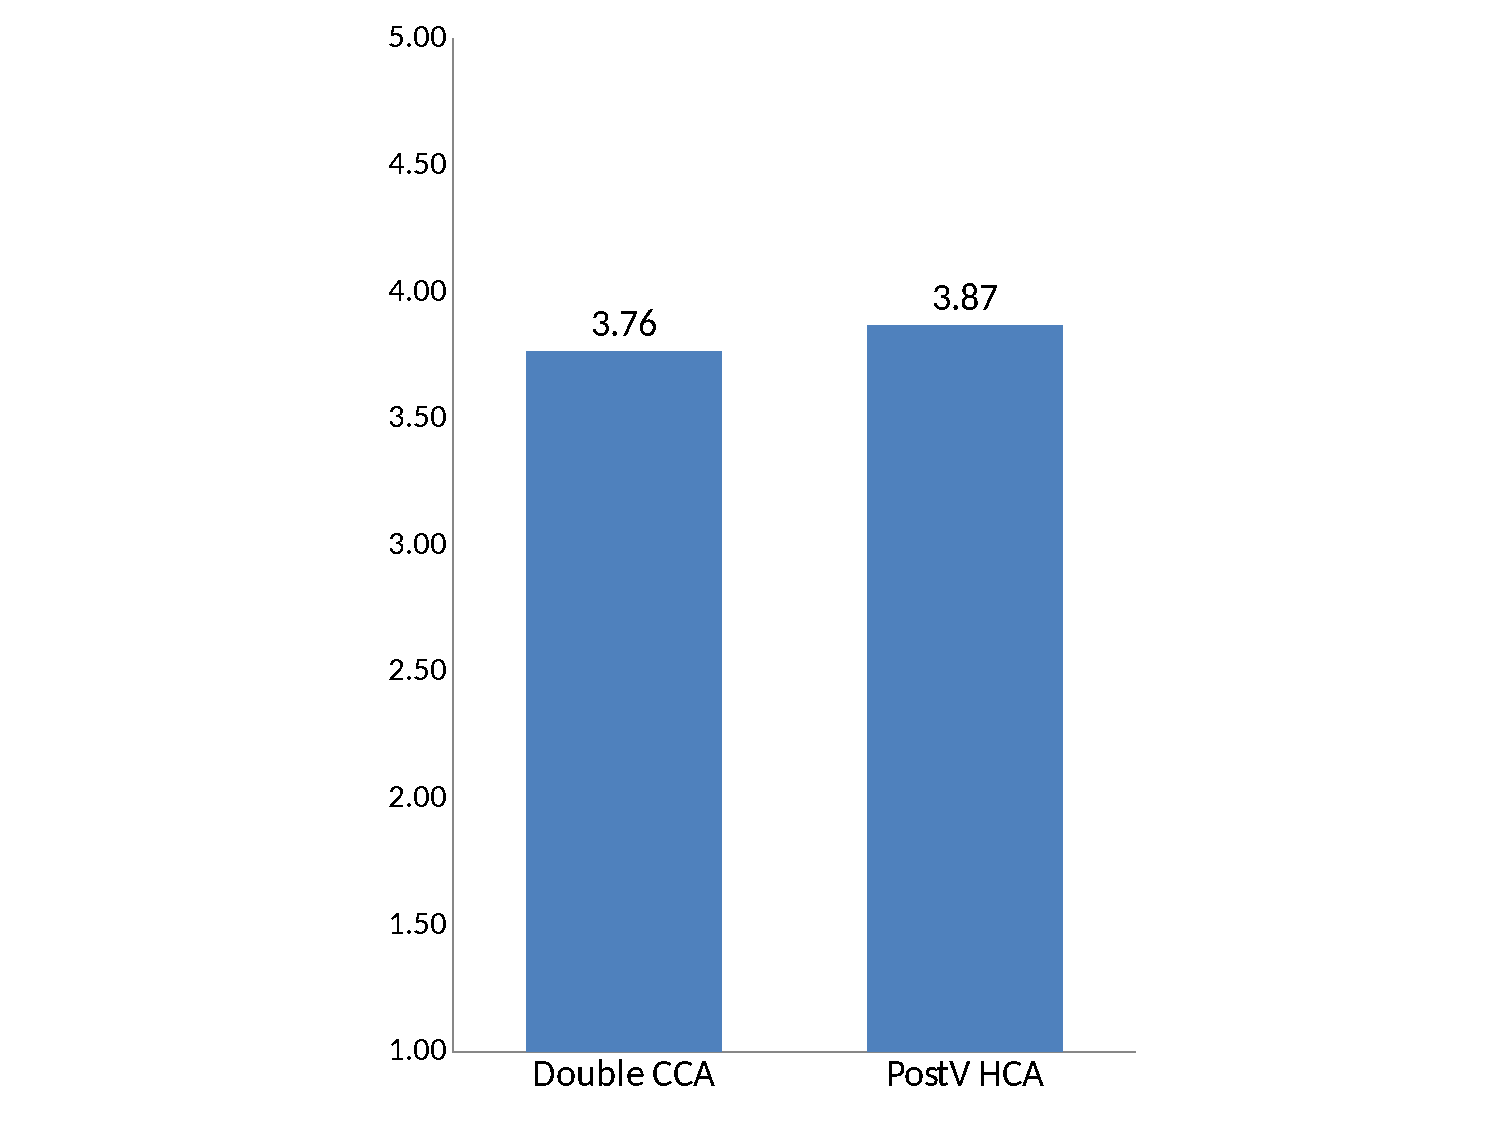
\includegraphics[height=200pt]{figures/cca_postv_nl.pdf}
\end{center}
\caption{Double closest conjunct agreement and Postverbal highest conjuct agreement, statistically indistinguishable}
\label{fig:figure_cca_postv}
\end{figure}

\subsection{Double CCA vs double HCA}
Double HCA -- in other words, the second participle agreeing with the first conjunct -- is still rated as acceptable, but to a much lesser degree than Double CCA.  Recall that the mechanism proposed in \citet{marusicnevinsbadecker:15} is that CCA vs HCA results from a choice in the ordering between Linearization and Agree-Copy, with the order of Linearization before Agree-Copy as preferred overall. This same preference carries over to sandwiched configurations. We have asserted that the choice of agreement Goal for each participle is independent, and in principle, the ordering of the operations of Linearization and Agree-Copy within a single derivation is, by hypothesis, variable, as shown in Table \ref{tab:order}. Note however, that should some principle of identical orderings across Probes within a single derivation (or domain) hold, then only the first and last rows of the table would be available.\footnote{Note further that if, for example, one assumed that Linearization occurs once only, but that Agree-Copy is enacted for each Probe at PF, proceeding bottom-up, then the second row of Table \ref{tab:order} would be impossible, as Part$_2$ could not be after Linearization and a higher, later probe be before Linearization.}

\begin{table}
\begin{tabularx}{\textwidth}{XXX} 
	\lsptoprule
Part$_1$'s Agree-Copy &  Part$_2$'s Agree-Copy &\\ \midrule
Before Linearization & Before Linearization & Double HCA\\ \midrule
Before Linearization & After Linearization& Double CCA\\ \midrule
After Linearization & Before Linearization& Double HCA\\ \midrule
After Linearization & After Linearization& Double CCA\\ 
\lspbottomrule
\end{tabularx}
\caption{Theoretically available options of ordering of Linearization and Agree-Copy}
\label{tab:order}
\end{table}
\newpage\noindent However, suppose that there is already a probability of speakers choosing CCA over HCA (i.e. of choosing a given Linearization ordering), say with p(CCA) $>$ p(HCA). In sandwiched configurations, while the probability of Double CCA would be reduced, at the same time, the probability of Double HCA should be reduced even more. 
The comparison of Double CCA vs Double HCA is shown in Figure \ref{fig:figure_cca_hca}, and their difference in means is statistically significant with a p-value $<$ 0.001.


\subsection{Double HCA vs HCA+Def}
We now turn to the next possibility with sandwiched configurations down in Table \ref{tab:sandwichoptions}, HCA+Def. Recall that Double CCA, Double HCA, and this strategy all involve the same surface target for Part$_1$ and differ only in the target chosen by Part$_2$. As it turns out, the ratings from Double HCA and HCA+Def are not different, indicating that, should we hold the postverbal choice to be independent from that of Part$_2$, then for preverbal subjects, HCA and Default agreement are 

\begin{figure}[h]
	\begin{center}
		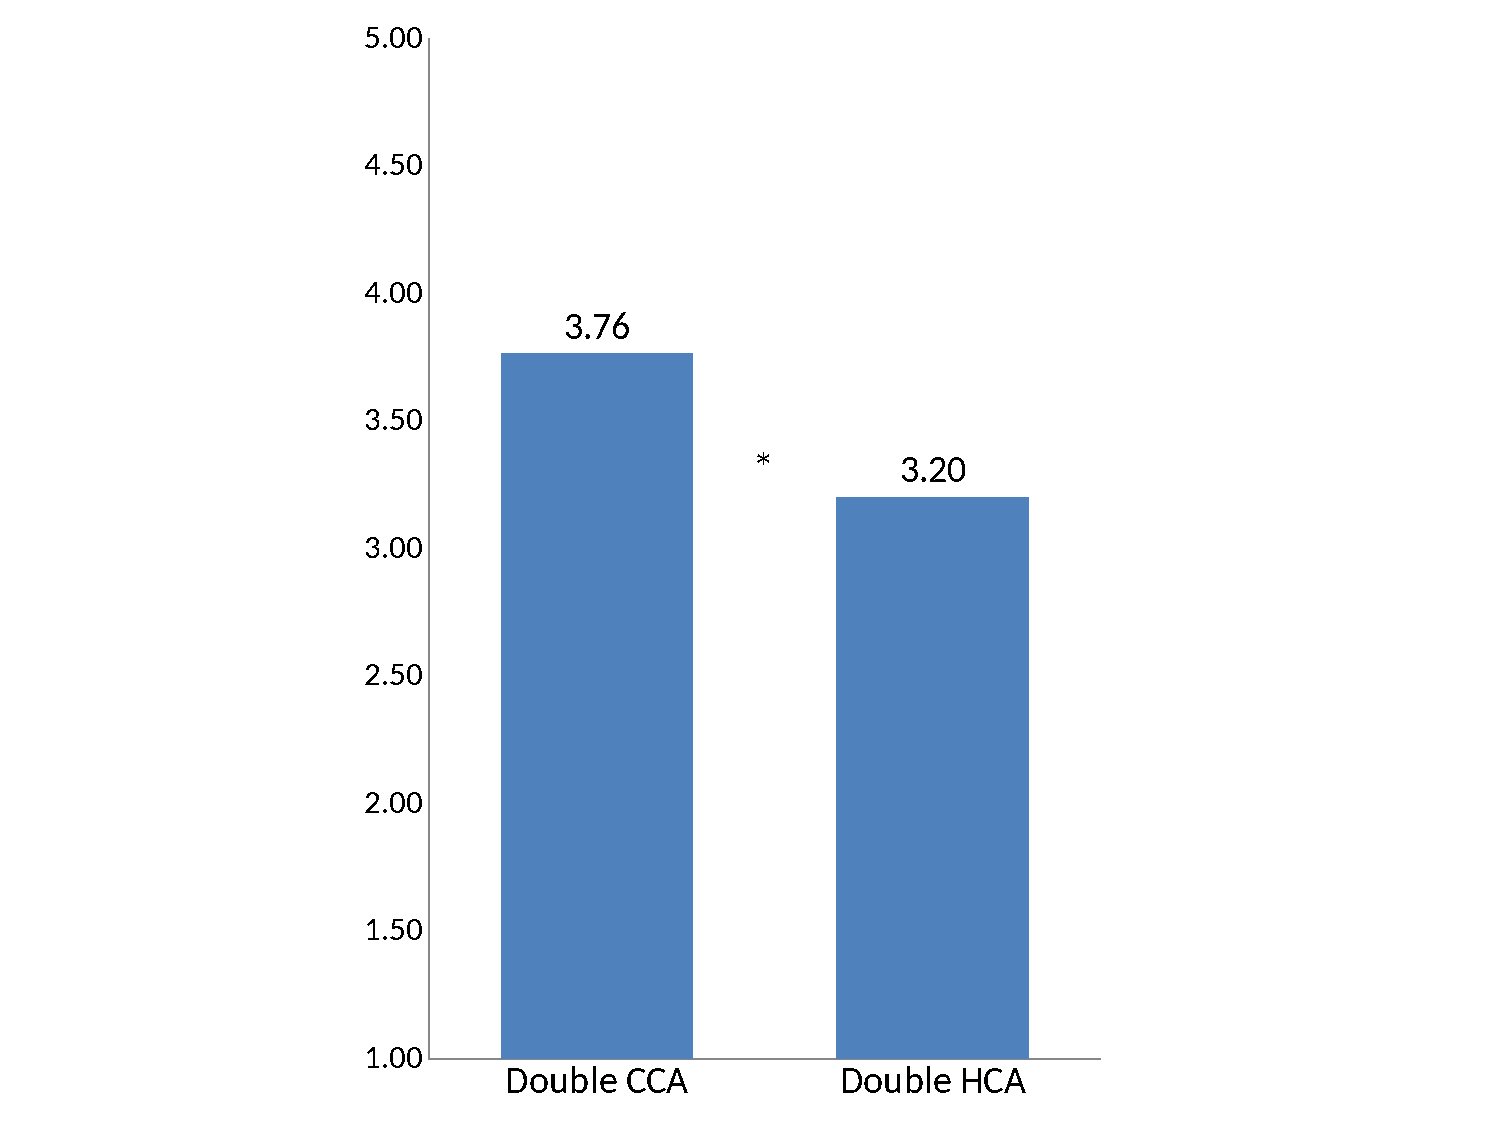
\includegraphics[height=200pt]{figures/cca_hca_nl.pdf}
	\end{center}
	\caption{Double closest conjunct agreement and Double highest conjunct agreement}
	\label{fig:figure_cca_hca}
\end{figure}
\newpage\noindent roughly of equal preference. These are not statistically different given the Bonferroni corrected p-value, as p $=$ .008, and are shown in Figure \ref{fig:figure_hca_hcadef}.\footnote{The difference between HCA+DEF and DEF+DEF (the latter which we take to be ungrammatical), is also statistically insignificant. The two conditions can nevertheless be grouped differently if we compare them to conditions  we take to be grammatical (because they are indistinguishable from our positive controls) and conditions we take to be bad (because they are indistinguishable from our negative controls). These groupings suggest these two conditions are not completely comparable, as HCA+DEF is simply put somewhere in the middle. We take HCA+DEF to be judged poorly also because default agreement in preverbal configurations in Slovenian is not a very strong option (as opposed to BCS; \citealt{willergold:16}). This may recall the initial option of `Peeking' grammars in \cite{marusicnevinsbadecker:15}, whereby the decision to allow default values at the \&P head is dispreferred to begin with. Confirming the validity of this analysis would require testing sandwiched configurations with one of the BCS language varieties where default agreement in simple preverbal configurations is judged equally good as CCA. We leave this for future work.}


\subsection{Postverbal default vs highest-default (DEF+DEF and DEF+CCA)} \label{sec:postverbaldef}
We now turn to two of the predicted unacceptable sandwiched configurations, namely the ones that involve postverbal default agreement on Part$_1$. According to the model herein, these should cause unacceptability regardless of the choice

\begin{figure}[h]
	\begin{center}
		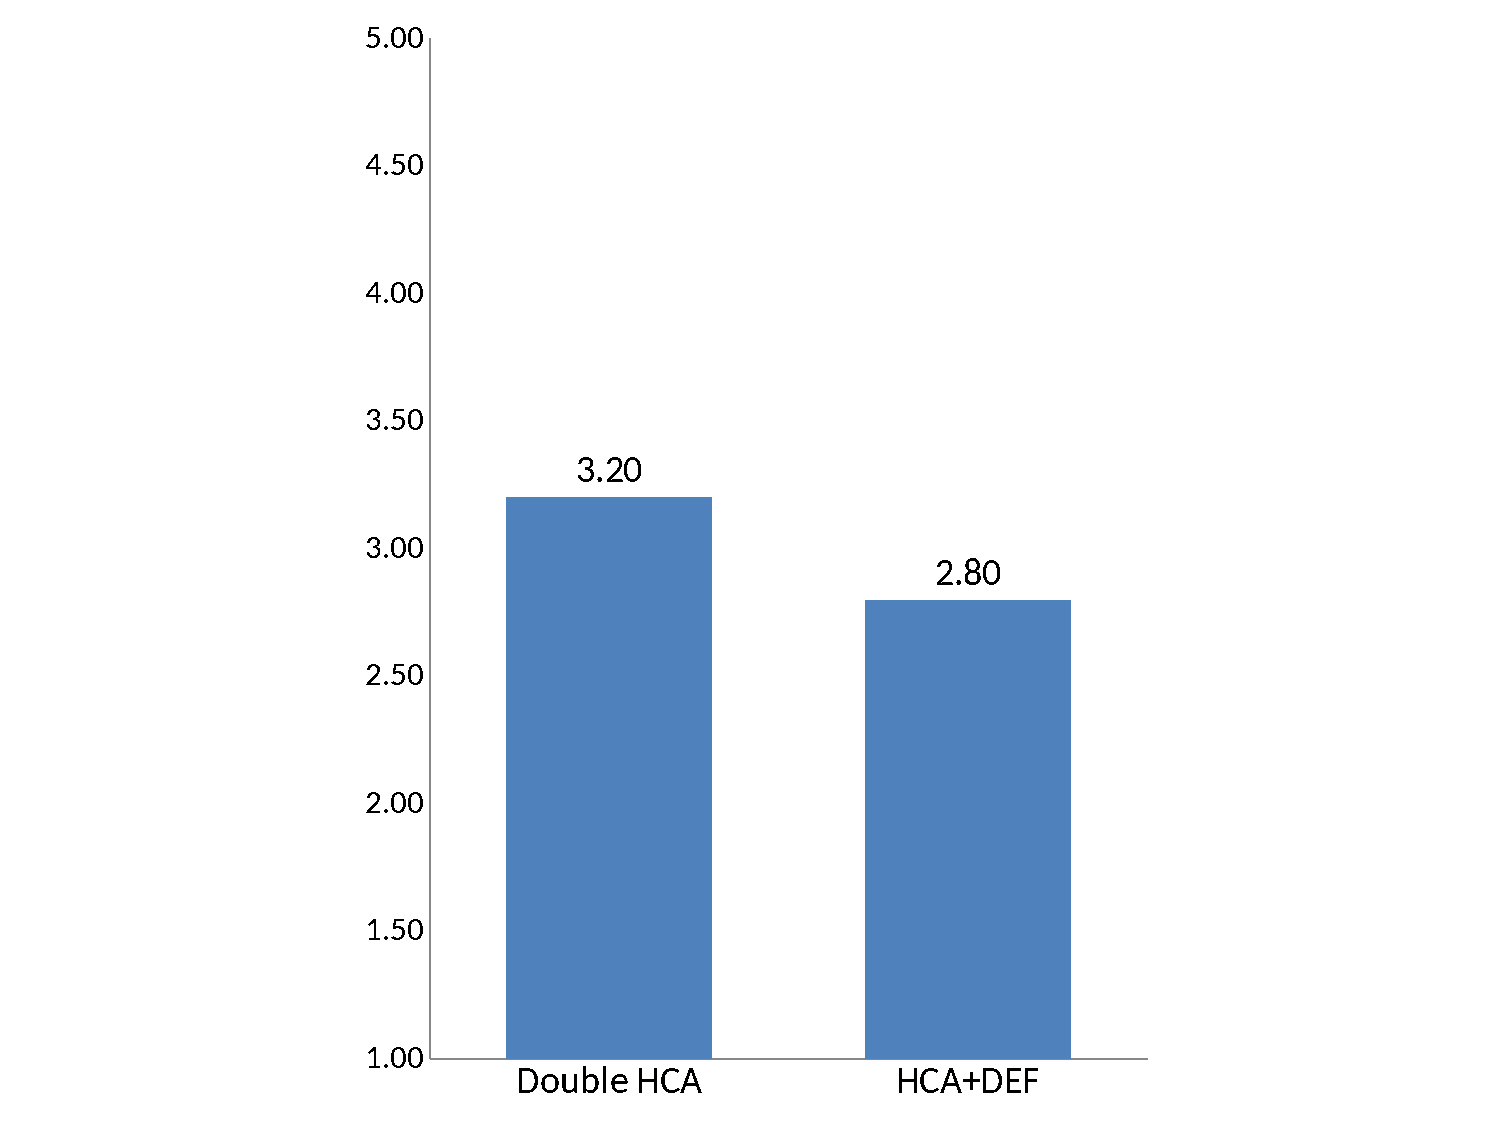
\includegraphics[height=200pt]{figures/hca_hcadef_nl.pdf}
	\end{center}
	\caption{Double Highest conjunct agreement compared with Highest conjunct agreement on the first participle with Default on the second participle element}
	\label{fig:figure_hca_hcadef}
\end{figure}
\noindent of agreement for Part$_2$. This prediction is indeed borne out, as both are not only rated low, but also are statistically indistinguishable from postverbal Default in a non-sandwiched configuration, a result already found to be degraded in \citet{willergold:16}. Thus, postverbal default is statistically indistinguishable from DEF+DEF (p = 0.009) and postverbal default is also indistinguishable from DEF+CCA: (p $>$ 0.5); all three are shown in Figure \ref{fig:figure_defdef_defcca_postvdef}.


\subsection{Postverbal LCA vs double LCA}
Our final condition examined was Double LCA, which was rated with a low acceptability (average rating 2.37). We left out of this experiment the control condition of Postverbal Lowest Conjunct agreement, as it has been reported impossible across a range of research discussing conjunct agreement in South Slavic (\citealt{marusicnevinsbadecker:15,boskovic:09,puskarmurphy:17,willergold:16}). Given the logic that what is available in simple pre- and postverbal cases is also available in sandwiched configurations, we would predict Double LCA to be just as bad as Postverbal LCA. Given that we did not test these two conditions in the same experiment, we cannot perform a statistical comparison 

\begin{figure}[h]
	\begin{center}
		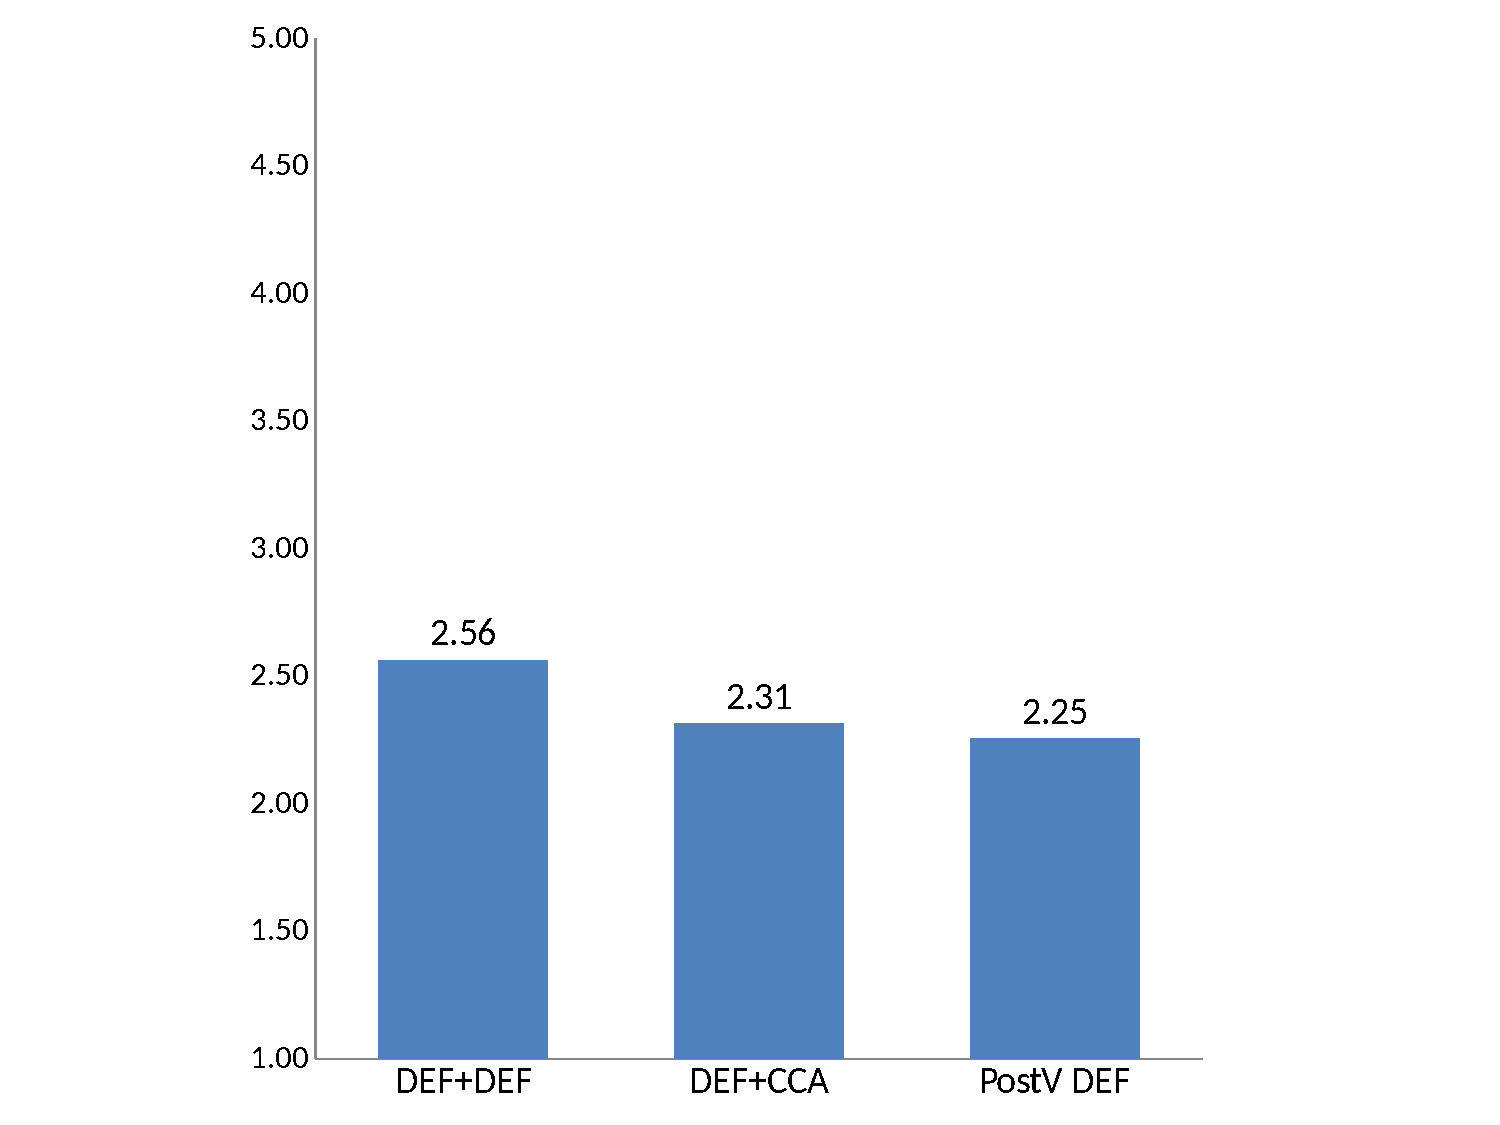
\includegraphics[height=200pt]{figures/defdef_defcca_postvdef_nl.pdf}
	\end{center}
	\caption{Double Default agreement vs. default on the first participle with closest conjunct agreement on the second participle vs. Postverbal default agreement}
	\label{fig:figure_defdef_defcca_postvdef}
\end{figure}
\noindent between the two, but as both were graded in principle as unavailable, we can still conclude our prediction is borne out also with this condition. Nonetheless, we can compare Double LCA vs Double HCA (p $<$ 0.0001) and Double LCA vs Double CCA (p $<$ 0.0001), as shown in Figure \ref{fig:figure_cca_hca_lca}. 



\section{Consequences for theoretical models}
%, Franks and Willer Gold 2012
We have presented experimental evidence that sandwiched configurations exist, and that linear order effects exist in agreement to the point where each participle flanking a conjunction can agree with a different individual conjunct. As we have shown in Slovenian, the highest rated pattern involves the higher verbal probe targeting the first conjunct while the lower verbal probe targets the lower conjunct. 

On the whole, the results are strikingly consistent with the predictions made in Table \ref{tab:sandwichoptions}. Placing Agree-Copy in PF makes the surface order in sandwiched configurations all that matters for determining Double CCA/HCA by the second participle, in terms of two derivational choices: whether default agreement is 

\begin{figure}[h]
	\begin{center}
		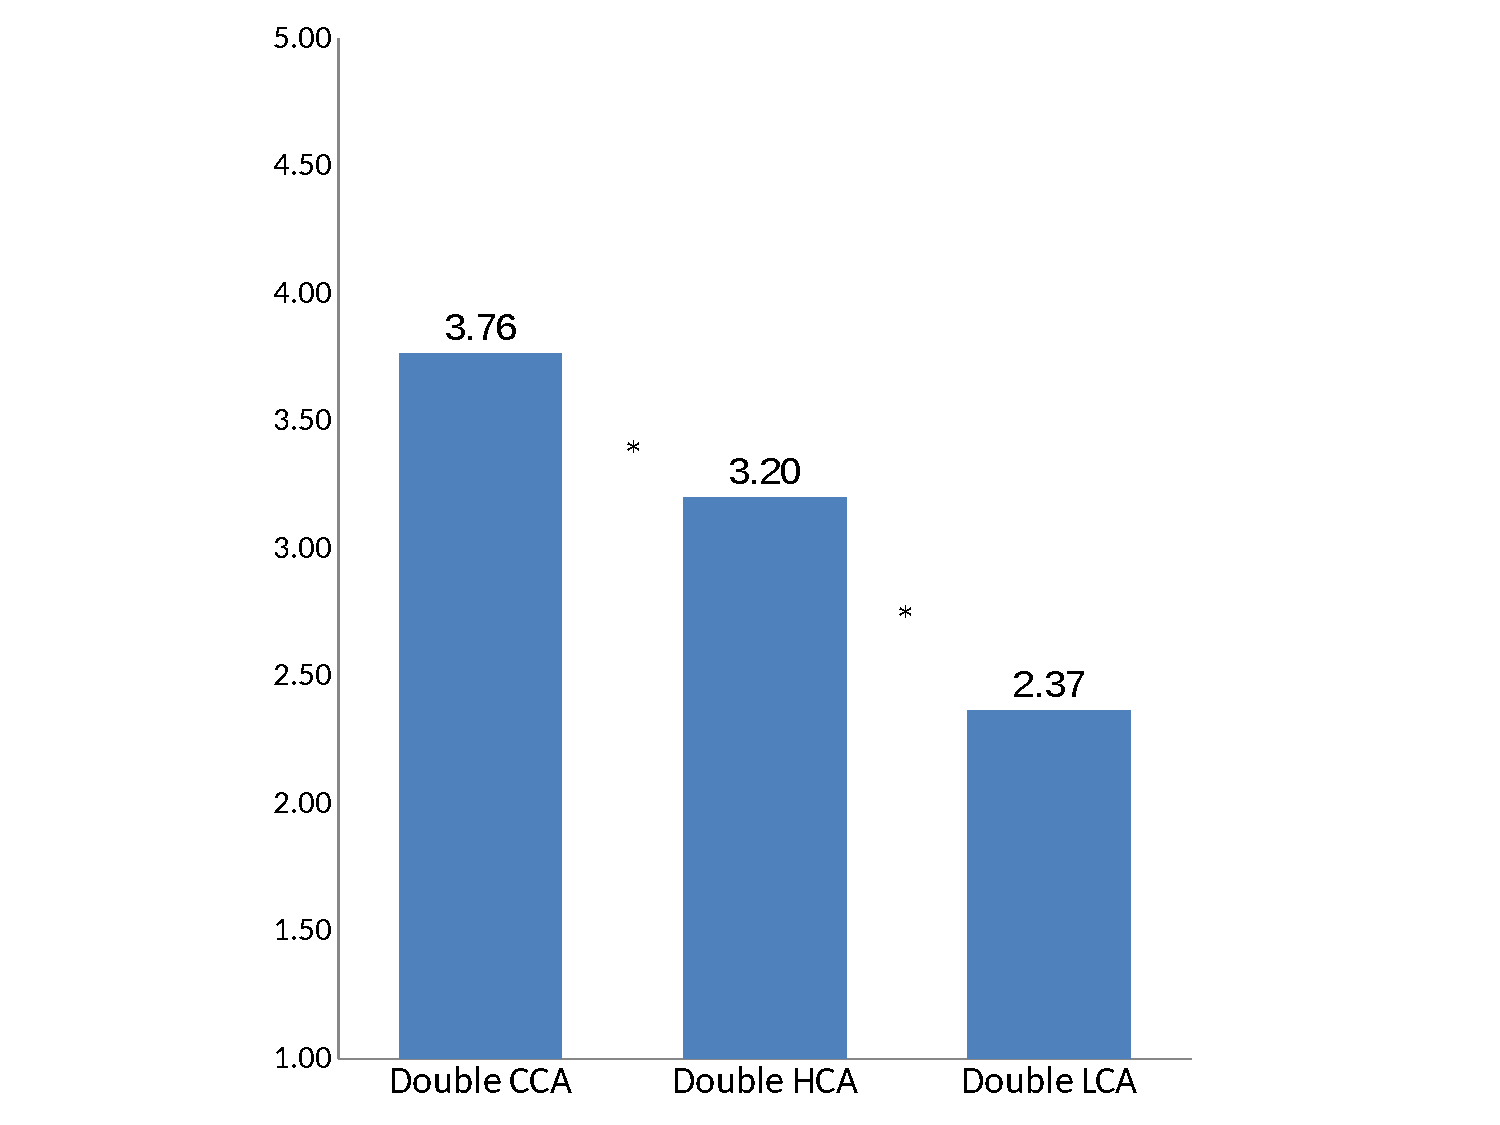
\includegraphics[height=200pt]{figures/cca_hca_lca_nl.pdf}
	\end{center}
	\caption{Double Closest conjunct agreement vs. Double highest conjunct agreement vs. Double lowest conjunct agreement}
	\label{fig:figure_cca_hca_lca}
\end{figure}
\noindent chosen (given the proviso that it can only be chosen when the subject \&P surface c-commands the participle) and whether Agree-Copy precedes or follows Linearization.

By contrast, other approaches to Conjunct agreement in South Slavic languages (cf. \citealt{boskovic:09,puskarmurphy:17}) derive CCA via syntactic mechanisms whereby all operations are restricted to narrow syntax. Concretely, \cite{boskovic:09} predicts highest conjunct agreement is impossible, as in order to derive Closest conjunct agreement he resorts to deletion of the features of the higher conjunct. Note that Highest conjunct agreement is not only available in regular conjunct agreement cases but has been found as a possible strategy also in sandwiched configurations. If the only way to derive Closest conjunct agreement is to delete the phi features of the first conjunct, then it should be completely impossible to get the most common agreement pattern --- Double CCA --- while the only available patterns should be the two agreement patterns that were graded to be worst --- Double LCA and DEF+CCA. \cite{puskarmurphy:17}, on the other hand, derive closest conjunct agreement from mechanisms internal to the \&P, which founders on cases where it seems that each individual Probe decides its own Goal from within the \&P. Although they add a mechanism of deactivation for Double CCA, this may end up in turn causing problems for Double HCA. Empirically, \cite{puskarmurphy:17} claim default agreement is available with postverbal subjects, which was empirically challenged in \cite{willergold:16} and here as well. Default agreement with postverbal subjects was the lowest rated pattern in this experiment. Finally, approaches that attempt to derive CCA via ellipsis would face clear challenges with Double CCA in sandwiched configurations, as it is wholly unclear what base unelided structure would underlie them.

The overall consistency of patterns found with these somewhat rare sandwiched configurations are of broader interest in that speakers presumably have very little exposure to such patterns but nonetheless arrive at clear results in how to compute agreement. This suggests that learning the interaction between Agree-Link and Agree-Copy with single-participle configurations can be readily extended to double-participle configurations with little or no modification to the existing set of operations, and confirm that a linearity-based approach to Agree-Copy is readily extended to more intricate constructions without necessarily needing to readjust the grammar for such cases. There are many additional empirical extensions of the present work that could be pursued, especially in comparison with other South Slavic varieties (specifically Bosnian/Croatian/Serbian), and with the additional sandwiched configurations discussed in Section \ref{sec:sandwconf}. Finally, it is worth noting that the present results were conducted in configurations in which both conjuncts in the \&P were plural. Extensions of the present work to combinations of different number, or indeed of double dual configurations in Slovenian, could prove worthwhile in further refining the current model.

% % % \nocite{introduction2019}

\section*{Abbreviations}

\begin{multicols}{2}
	\begin{tabbing}
		{HCA}\hspace{5mm} \= Highest conjunct agreement\kill
CCA \> Closest conjunct agreement\\
DEF \> Default agreement\\
F \> Feminine\\
HCA \> Highest conjunct agreement\\
LCA \> Lowest conjunct agreement\\
N \> Neuter\\
M \> Masculine\\
PF \> Phonological form\\
PL \> Plural\\
SG \> Singular\\
V \> Verb\\
3P \> third person\\
\&P \> Coordination Phrase
	\end{tabbing} 
\end{multicols}

\section*{Acknowledgements}
We would like to thank the editors, the audience at the Frankfurt agreement workshop, Boban Arsenijević, and Jana Willer Gold, Zorica Puškar, and Nadira Aljović. This research is partially funded by Leverhulme Trust Grant 512900 (to Nevins) and by Slovenian Research Agency Grant P6-0382 (to Marušič). 


{\sloppy\printbibliography[heading=subbibliography,notkeyword=this]}

\end{document}
